\documentclass[11pt]{standalone}

\usepackage{ifthen}
\usepackage{amsmath}
\usepackage{tikz} 
\usepackage[d]{esvect}
\usetikzlibrary{shapes.misc}
\usetikzlibrary{arrows,arrows.meta}
\usetikzlibrary{calc,intersections, patterns, math}

\definecolor{pfeil}{RGB}{168,167,167}
\definecolor{salmon}{RGB}{250,128,114}
\definecolor{petrol}{RGB}{0, 118, 136}
\definecolor{darkgoldenrod}{RGB}{184, 134, 11}
\colorlet{petrol-lighter}{petrol!40}
\colorlet{darkgoldenrod-lighter}{darkgoldenrod!40}

\begin{document}

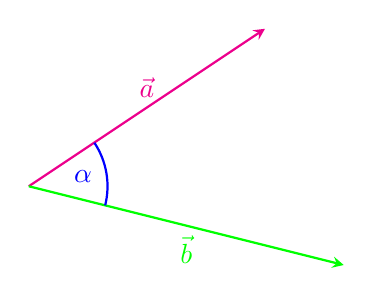
\begin{tikzpicture}[pfeil, >=stealth, very thick]
			
	\draw[thick,->,magenta] (0,0) -- node[above]{$\vec a$} (3,2);
	\draw[thick,->,green] (0,0) -- node[below]{$\vec b$} (4,-1);
	\draw[thick, blue] (-14.04:1) arc(-14.04:33.5:1);
	\node[blue] at (10:0.7) {$\alpha$};

\end{tikzpicture}			

\end{document}
